\section{Introduction}

The recommendation for a future state  for Rubin Observatory Operations documentation is presented in Project-wide Documentation Proposal for Rubin Observatory Operations, \citeds{SITCOMTN-014}. 
This document provides the migration plan for Rubin construction-era documentation into this future state documentation system. 
It includes a timeline for implementing the Documentation Portal\footnote{the  primary interface for searching and browsing all Rubin documentation, irrespective of which Rubin-adopted storage platform they reside on} and a transition plan to migrate construction-era  documentation deliverables to conform with the future state documentation strategy.
An estimate of the required resources is provided together with the responsibilities of each of the Rubin subsystems to ensure delivery of the future state documentation system by the start of LSST operations. 

This document fully addresses charge items 5 and 6 and partially addresses charge item 7 in the Charge to the Project-Wide Documentation Working Group \citeds{LSE-489}. 


\section{Transition Plan and Workflow}

Describe the process for transition from the current state to the future state.

Design a workflow

\section{Required Resources \& Subsystem Responsibilities}

Description of the estimated resources need to carry out this implementation plan and what the roles and responsibilities are for each subsystem in this context.

Need to take information from Storage View subsections, then find gaps to confirm add with DWG or identify potential gaps for project/departments/groups to consider.

The departments and technical groups are responsible; documentation specialists primary assistants; and both depend on system administrators and software developers on case-by-case need.
Transition Joint Work.

\begin{enumerate}
        \item Documentation Quantification
        \item Documentation Selection
        \item Proposed repositories Reviewing
        \item Starting and Finishing Scheduling
\end{enumerate}

Recommend new Operations Documentation Committee/Group for project-wide support, common tools and distributed development of them, lessons learned, etc.
Project-provided charge and scope.
Composition: documentation lead(s), documentation specialists, SQuaRE seat, ex-officio manager (department or subgroup?)
Need Chuck, Austin, Leanne input to min (and possibly max) bound level of effort for this role.

\begin{figure}[t]
\caption{Temporary Caption.}
\centering
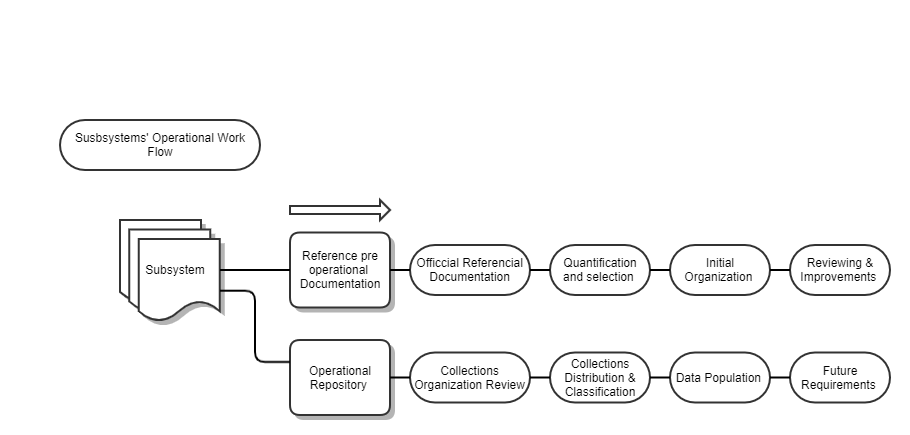
\includegraphics[width=\textwidth]{subsystems-role-workflow-temp}
\label{fig:subsystems-role-workflow}
\end{figure}

\begin{figure}[t]
\caption{Temporary Caption.}
\centering
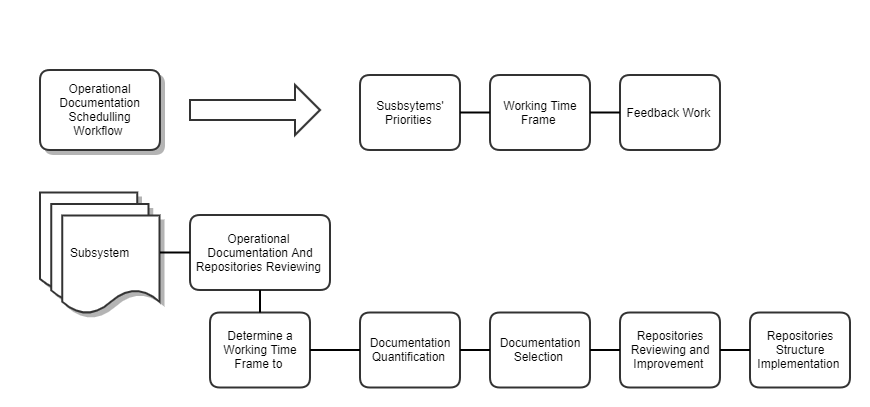
\includegraphics[width=\textwidth]{scheduling-workflow-temp}
\label{fig:scheduling-workflow}
\end{figure}

%%% Schedule  
\section{Schedule}

Outline the schedule needed for implementation to meet the objective delivering a coherent tachnical document packed at the end of the Project Construction effort.
Need to take information from Storage View subsections, then find gaps to confirm add with DWG or identify potential gaps for project/departments/groups to consider.


%%% Risk
\section{Risk Analysis}

A full risk assessment is not provided here. 
A full risk analysis will be carried out following the processes and procedures of the Rubin Risk Board \citeds{rdo-71} and identified Risks and Mitigations added to the Rubin Risk Register. 

At a high-level, the risk of not implementing the strategy presented in \citeds{SITCOMTN-014} by the start of the LSST will make discovery of essential documentation about the Rubin/LSST system difficult, compromising efficient operations and science. 


